\documentclass[11pt]{article}

%%%%%%%%%%%%%%%%%%%%%%%%%%%%%%%%%%%%%%%%%%%%%%%%%%%%%%%%%%%%%%%%%%%%%%%%%%%%%%%% FORMATTING OPTIONS
%%%%%%%%%%%%%%%%%%%%%%%%%%%%%%%%%%%%%%%%%%%%%%%%%%%%%%%%%%%%%%%%%%%%%%%%%%%%%%%%
\usepackage{caption}
\usepackage{color}
\usepackage{changepage}
\usepackage{enumitem}
\usepackage[margin=2cm]{geometry}
\usepackage{graphicx}
\usepackage{here}
\usepackage{natbib}
\usepackage{subcaption}
\usepackage{titlesec}
\usepackage{xcolor}

\definecolor{darkblue}{RGB}{0,0,140}
\usepackage[colorlinks=true, allcolors=darkblue]{hyperref}

\titlespacing{\section}{0pt}{1ex}{0ex}
\setlength{\parskip}{8pt}%
\setlength{\parindent}{0pt}%

\newcommand{\fullname}{Core RL Behavior Suite}
\newcommand{\shortname}{\texttt{bsuite}}
\newcommand{\github}{\url{github.com/deepmind/bsuite}}



%%%%%%%%%%%%%%%%%%%%%%%%%%%%%%%%%%%%%%%%%%%%%%%%%%%%%%%%%%%%%%%%%%%%%%%%%%%%%%%% USER POPULATED FIELDS
\newcommand{\version}{\texttt{bsuite2019}}
\newcommand{\fullreport}{\url{ADD-LINK-HERE}}



%%%%%%%%%%%%%%%%%%%%%%%%%%%%%%%%%%%%%%%%%%%%%%%%%%%%%%%%%%%%%%%%%%%%%%%%%%%%%%%% DOCUMENT START
%%%%%%%%%%%%%%%%%%%%%%%%%%%%%%%%%%%%%%%%%%%%%%%%%%%%%%%%%%%%%%%%%%%%%%%%%%%%%%%%

\title{
\vspace{-20mm}
\rule{\linewidth}{4pt}
\vskip 1mm
\fullname: \shortname\ report
\vskip -6mm
\rule{\linewidth}{1pt}
\vskip -20mm
}
\date{}
\author{}

% \newcommand{\@toptitlebar}{
%   \hrule height 4\p@
%   \vskip 0.25in
%   \vskip -\parskip%
% }
% \newcommand{\@bottomtitlebar}{
%   \vskip 0.29in
%   \vskip -\parskip
%   \hrule height 1\p@
%   \vskip 0.09in%
% }

\begin{document}

\maketitle


%%%%%%%%%%%%%%%%%%%%%%%%%%%%%%%%%%%%%%%%%%%%%%%%%%%%%%%%%%%%%%%%%%%%%%%%%%%%%%%% ABSTRACT
{\small
\begin{adjustwidth}{1.5cm}{1.5cm}
The \textit{\fullname}, or \shortname\ for short, is a collection of carefully-designed experiments that investigate core capabilities of a reinforcement learning (RL) agent.
The aim of the \shortname\ project is to collect clear, informative and scalable problems that capture key issues in the design of efficient and general learning algorithms and study agent behaviour through their performance on these shared benchmarks.
This report provides a snapshot of performance on \version, obtained by running the experiments from \github\ \cite{osband2019bsuite}.
\end{adjustwidth}
}

%%%%%%%%%%%%%%%%%%%%%%%%%%%%%%%%%%%%%%%%%%%%%%%%%%%%%%%%%%%%%%%%%%%%%%%%%%%%%%%% AGENT DEFINITION
\section{Agent definition}
In this experiment all implementations are taken from \url{github.com/deepmind/bsuite/baselines}. \\
We provide a brief summary of the agents run on \version:
\vspace{-2mm}
\begin{itemize}[noitemsep, nolistsep]
    \item actor\_critic\_rnn: an actor critic with recurrent neural network \cite{gittins1979bandit}.
    \item boot\_dqn: bootstrapped DQN with prior networks \cite{osband2016deep,osband2018rpf}.
    \item dqn: Deep Q-networks \cite{mnih2015human}.
    \item random: selects action uniformly at random each timestep.
\end{itemize}



%%%%%%%%%%%%%%%%%%%%%%%%%%%%%%%%%%%%%%%%%%%%%%%%%%%%%%%%%%%%%%%%%%%%%%%%%%%%%%%% PLOTS
\section{Summary scores}

Each \shortname\ experiment outputs a summary score in [0,1].
We aggregate these scores by according to key experiment type, according to the standard analysis notebook.
A detailed analysis of each of these experiments may be found in a notebook hosted on Colaboratory: \fullreport.


\begin{figure}[h!]
\centering
\begin{subfigure}{.45\textwidth}
  \centering
  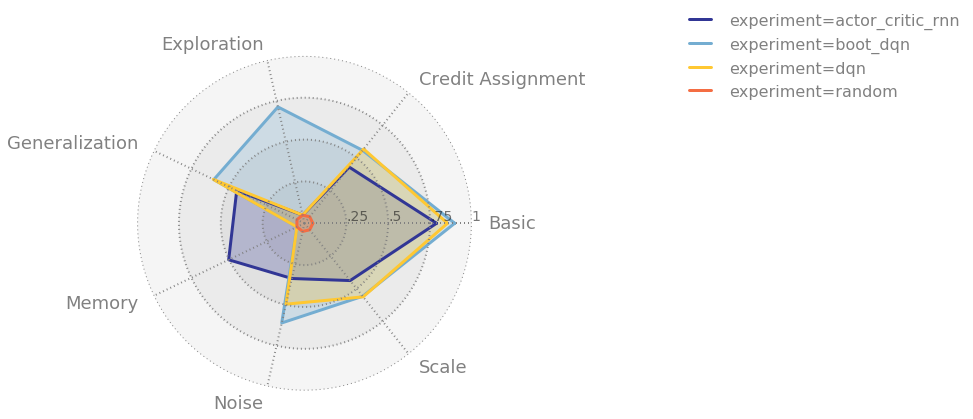
\includegraphics[width=95mm,height=60mm,keepaspectratio]{images/radar_plot}
  \caption{Radar plot for snapshot of agent characteristics.}
  \label{fig:memory_len_score}
\end{subfigure}
\hspace{10mm}
\begin{subfigure}{.45\textwidth}
  \centering
  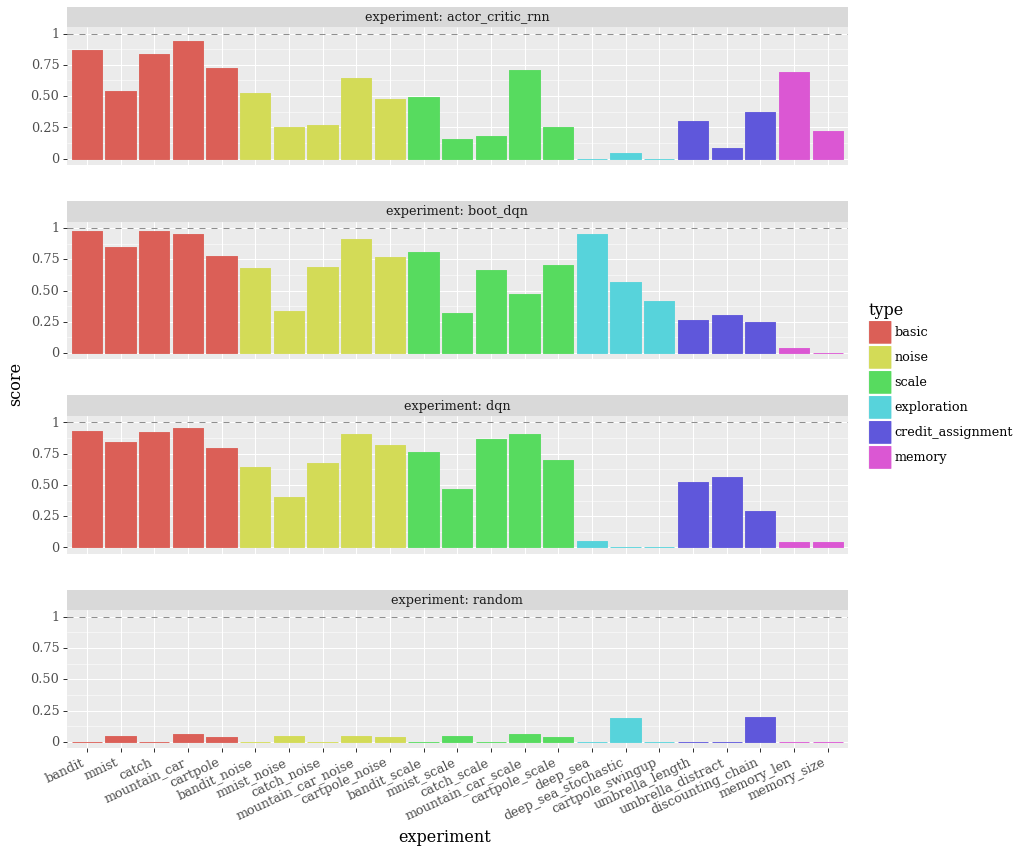
\includegraphics[width=95mm,height=60mm,keepaspectratio]{images/bar_plot}
  \caption{Examining score by individual experiment.}
  \label{fig:memory_len_scaling}
\end{subfigure}
\caption{Summary output from the \version\  experiments.}
\label{fig:test}
\end{figure}


%%%%%%%%%%%%%%%%%%%%%%%%%%%%%%%%%%%%%%%%%%%%%%%%%%%%%%%%%%%%%%%%%%%%%%%%%%%%%%%% KEY TAKEAWAYS
\section{Results commentary}
Here we have a small section where you can write some explanatory text.
Here we have a small section where you can write some explanatory text.
Here we have a small section where you can write some explanatory text.
Here we have a small section where you can write some explanatory text.
Here we have a small section where you can write some explanatory text.
Here we have a small section where you can write some explanatory text.
Here we have a small section where you can write some explanatory text.
Here we have a small section where you can write some explanatory text.



\newpage
%%%%%%%%%%%%%%%%%%%%%%%%%%%%%%%%%%%%%%%%%%%%%%%%%%%%%%%%%%%%%%%%%%%%%%%%%%%%%%%%%%% BIBLIOGRAPHY
%%%%%%%%%%%%%%%%%%%%%%%%%%%%%%%%%%%%%%%%%%%%%%%%%%%%%%%%%%%%%%%%%%%%%%%%%%%%%%%%%%%
{
\small
\bibliographystyle{plain}
\bibliography{../references}
}


\end{document}
